\documentclass{article}

\usepackage[a4paper, total={6.5in, 10in}]{geometry}
\usepackage{multicol}
 \usepackage{graphicx}
 \usepackage[export]{adjustbox}
 \usepackage{hyperref}

\usepackage{polyglossia}
\setmainlanguage{russian}
\setotherlanguage{english}

\setmainfont[Ligatures=TeX]{CMU Serif}
\setmonofont[Ligatures=TeX]{CMU Typewriter Text}

% Отключение нумерации
\pagenumbering{gobble}

% Межстрочный интервал
\renewcommand{\baselinestretch}{1.3}

\begin{document}

\begin{figure}
	\begin{minipage}{0.48\textwidth}
		\textbf{\Large{Шишканов Павел}}

		\large{Java backend-разработчик, 26 лет}
	\end{minipage}		
	\begin{adjustbox}{minipage=11cm, right}
		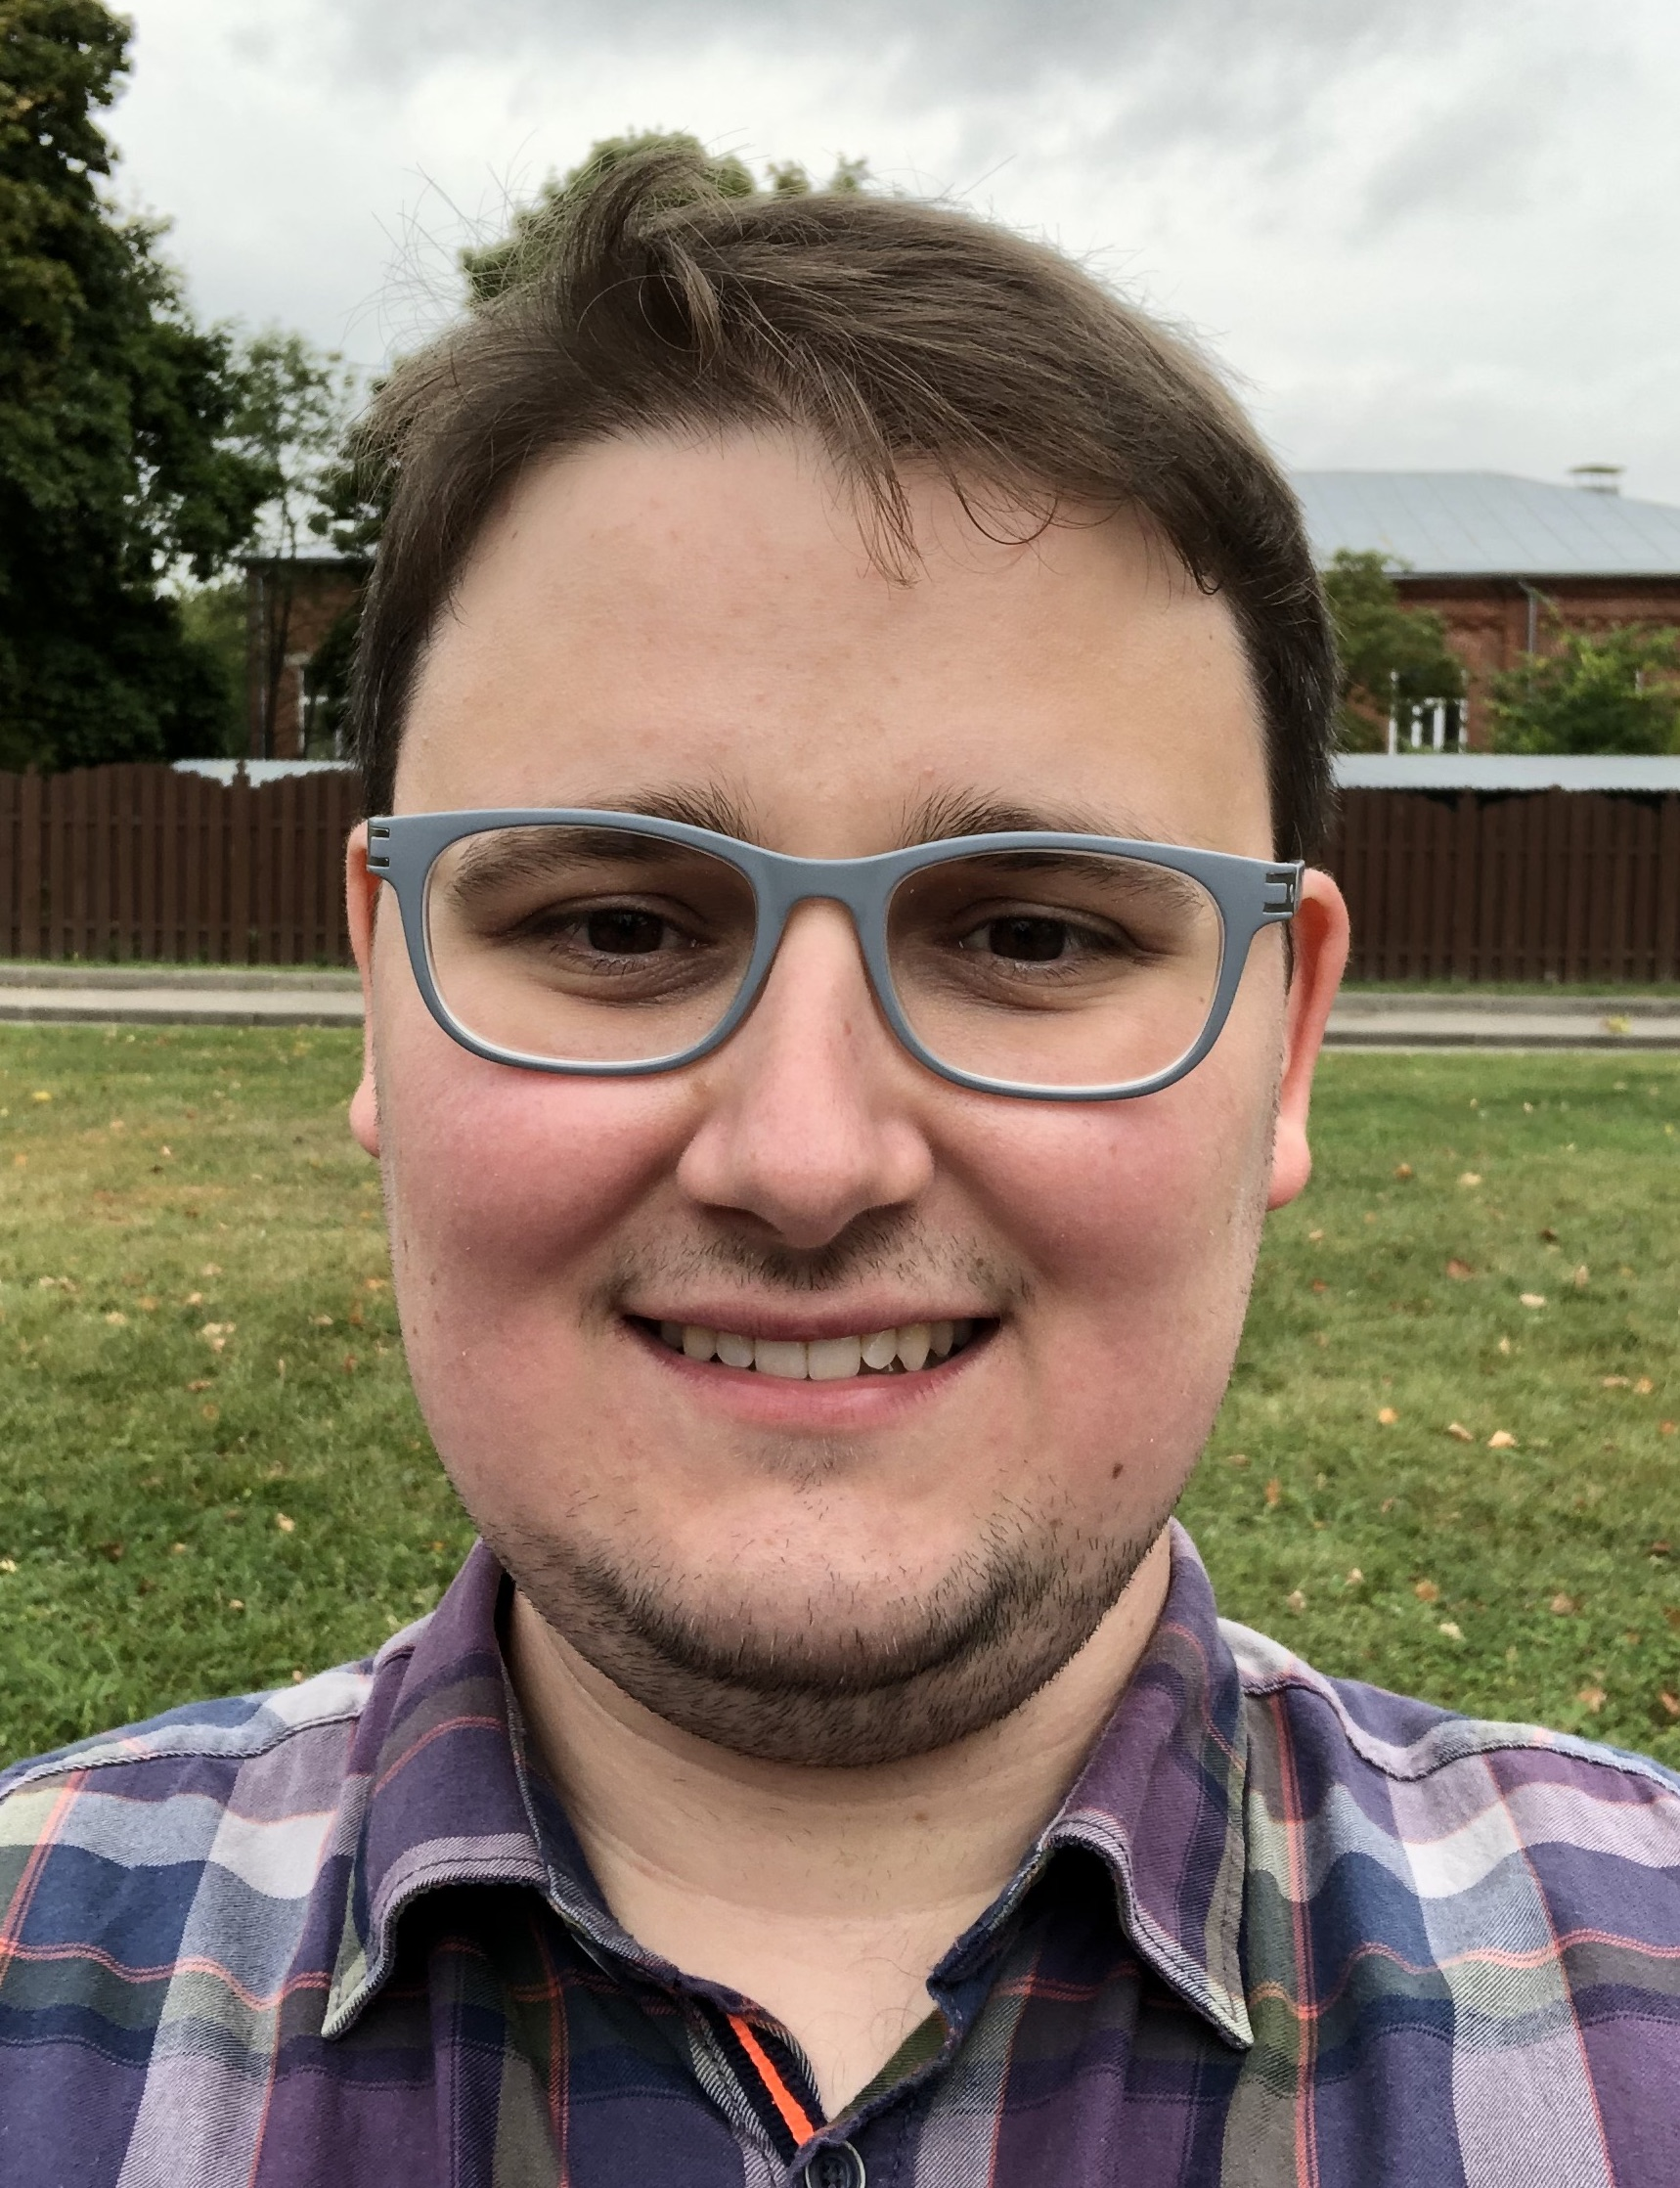
\includegraphics[scale=0.05]{logo.jpeg}
	\end{adjustbox}		
\end{figure}

\noindent\rule{\textwidth}{0.5pt}

\begin{multicols}{2}

\textbf{Локация:} Россия, г. Владимир

\textbf{Языки:} русский, английский / B1

\columnbreak

\textbf{Mobile:} \texttt{+79065621667}

\textbf{Email:} \texttt{pshishkanov@fastmail.com}

\end{multicols}

Backend-разработчик со стажем работы 6 лет. Имею опыт работы с крупными заказчиками в сфере финтеха (<<БКС>>, <<ВТБ>>, <<Nymbus>>) на стеке Java-технологий. Участвую во многих этапах решения задач, включая их анализ, проектирование и разработку.
Ищу работу с интересными бизнес-задачами в области высоконагруженных или низкоуровневых систем.

\noindent\rule{\textwidth}{0.5pt}

\Large{\textbf{Навыки:}}

\normalsize{

\begin{itemize}	
	\item Java и JVM (Kotlin, Spring Framework/Boot, Maven)
	\item Databases (Oracle DB, PostgreSQL)
	\item DevOps (Docker, Jenkins)
	\item Git
\end{itemize}

}

\noindent\rule{\textwidth}{0.5pt}

\Large{\textbf{Опыт работы:}}

\normalsize{

\begin{itemize}

	\item \textbf{февраль 2020 - май 2020} --- <<BSC Msc>> --- старший разработчик.

	Проект <<ВТБ>> (серверная часть мобильного банка <<ВТБ>>):

	\begin{itemize}		
		\item разработал аутентификацию и авторизацию для внутреннего приложения через LDAP over SSL;
		\item разработал универсальный mock для внутренних приложений с поддержкой работы по HTTP и SOAP;
		\item используемые технологии: Kotlin, Spring Framework 5, Spring Boot 2, PostgreSQL.
	\end{itemize}

	\item \textbf{январь 2018 - февраль 2020} --- <<BSC Msc>> --- разработчик.

	Проект <<NYMBUS>> (платформа дистанционного банковского обслуживания <<NYMBUS>>):

	\begin{itemize}		
		\item реализовал интеграцию с внешними сервисами для получения данных о банковских отделениях (получение данных из нескольких источников и их кеширование);
		\item доработал и настроил аутентификацию пользователей по TouchID/FaceID и по PIN;
		\item тестировал задачи через интеграционные тесты и реализовал утилиту для нагрузочного тестирования;
		\item написал пайплайны для Jenkins (сборка контейнеров с приложением, запуск интеграционных тестов, деплой на тестовое окружение);
		\item используемые технологии: Java 8/11, Spring Framework 4, Spring Boot, Oracle DB, REST API, SOAP, Docker, Jenkins.
	\end{itemize}

	\item \textbf{февраль 2016 - январь 2018} --- <<BSC Msc>> --- разработчик.

	Проект <<БКС>> (личный кабинет пользователя в интернет-банке <<БКС>>):

	\begin{itemize}		
		\item доработал личный кабинет пользователя (подключение торговых терминалов, подписание документов электронной подписью);
		\item реализовал микросервис для аутентификации и авторизации пользователей;
		\item используемые технологии: Java 7, Spring Framework 3, Tomcat, Oracle DB, JSP.
	\end{itemize}

	\item \textbf{март 2014 - февраль 2016} --- <<BSC Msc>> --- младший разработчик.

	Проект <<МИР>> (система управления обеспечением по сделкам с ценными бумагами в <<НРД>>):

	\begin{itemize}		
		\item разработал подсистемы для интеграции с разными источниками данных: прямая вставка данных в БД и пуллинг изменений, импорт данных в формате XML или CSV, обработка сообщений из брокера сообщений;
		\item написал XSLT-шаблоны для генерации репозитарных документов в формате XML;
		\item доработал графический интерфейс системы на базе фреймворка Wicket;
		\item используемые технологии: Java 6, WebSphere, MS SQL, Rabbit MQ, Wicket, SVN.
	\end{itemize}

\end{itemize}
}

\noindent\rule{\textwidth}{0.5pt}

\Large{\textbf{Образование:}}

\normalsize{

\begin{itemize}

	\item магистратура --- \textbf{сентябрь 2015 - июнь 2017} --- <<Владимирский государственный университет>>

	\begin{itemize}		
		\item специальность: <<Программная инженерия>>;
		\item дипломная работа: <<Разработка программного модуля для передачи потокового контента с использованием p2p-технологий>> (\href{https://github.com/pshishkanov/watch-stream-paper}{https://github.com/pshishkanov/watch-stream-paper}).
	\end{itemize}

	\item бакалавриат --- \textbf{сентябрь 2011 - июнь 2015} --- <<Владимирский государственный университет>>

	\begin{itemize}		
		\item специальность: <<Информационные системы и технологии>>;
		\item дипломная работа: <<Информационная система дистанционного обучения. Модуль проверки на плагиат>> (\href{https://github.com/pshishkanov/sherlock-paper}{https://github.com/pshishkanov/sherlock-paper}).		
	\end{itemize}

\end{itemize}
}

\end{document}